\chapter{Préparation du corpus}

L'objectif de ce premier TD est de construire un fichier XML unique et structuré à partir des fichiers HTML bruts de l'archive ADIT, afin de disposer d'une base propre et homogène pour toutes les étapes d'indexation qui suivront.

\section{Présentation des fichiers}

L'archive est constituée de bulletins électroniques publiés entre 2011 et 2014. Chaque bulletin est un fichier HTML contenant un ou plusieurs articles, répartis dans des rubriques telles que \textit{Focus}, \textit{Événement}, \textit{Actualité Innovation} ou \textit{En direct des laboratoires}. On souhaite en extraire les champs suivants : le numéro de l'article et du bulletin, la date de parution, la rubrique, le titre, le texte, l'auteur, les images avec leur URL et leur légende, et les informations de contact.

\section{Extraction des champs à partir du HTML}

\subsection{Architecture du parseur}

On structure le parseur autour de deux classes aux responsabilités distinctes. \texttt{BulletinParser} prend en charge un unique fichier HTML : il l'ouvre, en extrait tous les champs, et produit le fragment XML correspondant. \texttt{CorpusParser} orchestre l'ensemble : il itère sur tous les fichiers du répertoire, instancie un \texttt{BulletinParser} par fichier, puis assemble les fragments pour produire le fichier \texttt{corpus.xml}.

\subsection{Double parsing du HTML}

On commence par passer chaque fichier dans \texttt{BeautifulSoup} pour normaliser le HTML potentiellement malformé, puis on transmet le résultat à \texttt{etree.HTML()} de \texttt{lxml} pour obtenir un DOM interrogeable en XPath. Cette combinaison tire parti de la robustesse de BeautifulSoup pour la correction du HTML et de l'expressivité de XPath pour l'extraction des champs.

\subsection{Extraction par chemins XPath}

Tous les champs sont ciblés par des chemins XPath identifiés en inspectant la structure HTML depuis le navigateur. On applique \texttt{strip()} sur les valeurs extraites pour nettoyer les espaces parasites, et \texttt{replace()} pour isoler certaines informations encodées dans le texte, comme le numéro de bulletin toujours précédé de la chaîne \texttt{"BE France"}.

\textbf{Extraction du texte.} Le texte de l'article partage la même cellule HTML que les images. Pour n'extraire que le contenu éditorial, on utilise un prédicat XPath qui exclut les blocs contenant des images (\texttt{not(ancestor::div[img])}) et les spans de légende (\texttt{style88}).

\textbf{Extraction des images.} Les images sont ciblées via \texttt{div[img]}, l'URL récupérée via l'attribut \texttt{src}, et la légende via \texttt{following-sibling::span}.

\textbf{Extraction de l'auteur.} Le bloc auteur suit la forme \texttt{Organisation - Nom - Email : adresse}. Une expression régulière souple avec \texttt{re.IGNORECASE} en extrait les trois sous-champs. En cas d'échec, les champs sont mis à \texttt{None} plutôt que de lever une exception, afin de ne pas interrompre le traitement des autres articles.

\textbf{Contact.} La structure du bloc contact étant trop hétérogène, on l'inclut tel quel dans la balise \texttt{<contact>} du XML.

\section{Construction du fichier XML et de l'index}

\subsection{Formation du fichier XML}

Chaque \texttt{BulletinParser} produit un fragment XML que \texttt{CorpusParser} accroche à la racine \texttt{<corpus>}. Chaque article est encapsulé dans une balise \texttt{<document>}, conformément à la structure imposée par le TD. L'ensemble est consolidé dans le fichier \texttt{clean\_corpus.xml}.

\subsection{Tokenisation}

La tokenisation est assurée par \texttt{CorpusTokenizer}. On segmente uniquement sur les espaces et les apostrophes, ce qui \textbf{conserve le tiret} à l'intérieur des tokens (\texttt{bien-être} reste un token unique, préservant ainsi les termes composés). Chaque token est mis en minuscules, et tous les caractères spéciaux sont supprimés à l'exception de \texttt{\textbackslash w} et du tiret. Les chiffres sont conservés pour permettre la détection des entités numériques au TD4. Enfin, le titre et le texte sont \textbf{concaténés avant tokenisation}, de sorte que le titre contribue à la fréquence globale des tokens pour le calcul du TF-IDF.

\subsection{Construction de l'index inversé}

Les fichiers inverses sont construits par la classe \texttt{Index} depuis le script \texttt{make\_index.py}. La méthode \texttt{build()} distingue les \textbf{champs tokenisés} (\texttt{titre}, \texttt{texte}), découpés par \texttt{CorpusTokenizer} et indexés avec leur fréquence et la liste des documents associés, des \textbf{champs bruts} (\texttt{rubrique}, \texttt{bulletin}, \texttt{date}, \texttt{auteur}, \texttt{contact}), mis en minuscules et indexés tels quels pour permettre une correspondance exacte. La présence d'images est indexée via le token \texttt{"image"} dès qu'une balise \texttt{<images>} est détectée. Les résultats sont sauvegardés en TSV, un fichier par section, ainsi qu'un fichier \texttt{lemmes\_corpus.csv} consolidant l'ensemble des tokens uniques.

\begin{figure}[h]
    \centering
    \hspace*{-0.1\textwidth}
    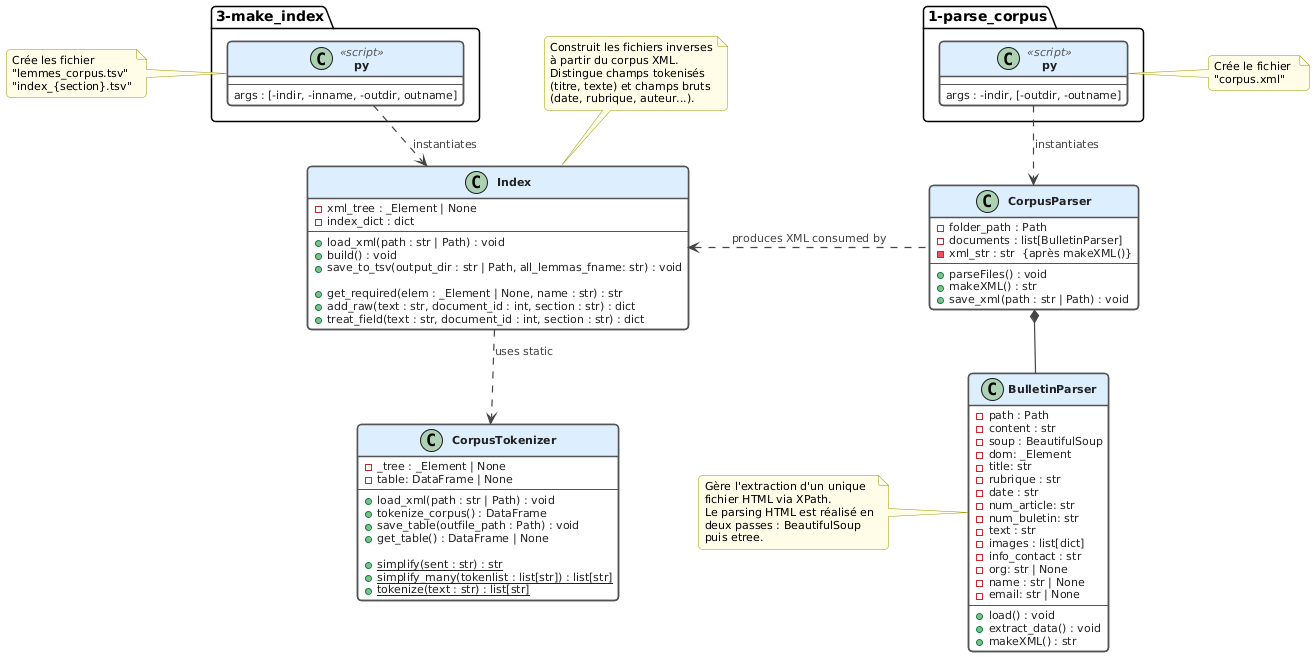
\includegraphics[width=1.2\textwidth]{assets/1-Index.png}
    \caption{UML Indexation (TD1)}
    \label{fig:TD1-Index}
\end{figure}
